\chapter{Benchmark configurations}
\label{app:benchmarks}

\begin{figure}[h]
	\centering
	\begin{subfigure}{.2\textwidth}
		\centering
		\includegraphics[width=.8\textwidth]{imgs/estee/shapes/plain}
		\caption{}
		\label{fig:tg-plain}
	\end{subfigure}%
	\begin{subfigure}{.2\textwidth}
		\centering
		\includegraphics[width=.8\linewidth]{imgs/estee/shapes/fork}
		\caption{}
		\label{fig:tg-fork}
	\end{subfigure}
	\begin{subfigure}{.2\textwidth}
		\centering
		
\includegraphics[width=.8\linewidth]{imgs/estee/shapes/fork2}
		\caption{}
		\label{fig:tg-fork2}
	\end{subfigure}
	\begin{subfigure}{.2\textwidth}
		\centering
		
\includegraphics[width=.8\linewidth]{imgs/estee/shapes/v}
		\caption{}
		\label{fig:tg-v}
	\end{subfigure}
	\\
	\begin{subfigure}{.2\textwidth}
		\centering
		
\includegraphics[width=.8\linewidth]{imgs/estee/shapes/w}
		\caption{}
		\label{fig:tg-w}
	\end{subfigure}
	\begin{subfigure}{.2\textwidth}
		\centering
		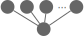
\includegraphics[width=.8\linewidth]{imgs/estee/shapes/merge}
		\caption{}
		\label{fig:tg-merge}
	\end{subfigure}
	\begin{subfigure}{.2\textwidth}
		\centering
		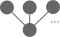
\includegraphics[width=.8\linewidth]{imgs/estee/shapes/merge-triplets}
		\caption{}
		\label{fig:tg-merge-triplets}
	\end{subfigure}
	\begin{subfigure}{.2\textwidth}
		\centering
		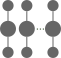
\includegraphics[width=.8\linewidth]{imgs/estee/shapes/triplets}
		\caption{}
		\label{fig:tg-triplets}
	\end{subfigure}
	\\
	\begin{subfigure}{.2\textwidth}
		\centering
		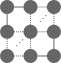
\includegraphics[width=.8\linewidth]{imgs/estee/shapes/grid}
		\caption{}
		\label{fig:tg-grid}
	\end{subfigure}
	\begin{subfigure}{.2\textwidth}
		\centering
		\includegraphics[width=.8\linewidth]{imgs/estee/shapes/splitters}
		\caption{}
		\label{fig:tg-splitters}
	\end{subfigure}
	\begin{subfigure}{.2\textwidth}
		\centering
		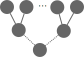
\includegraphics[width=.8\linewidth]{imgs/estee/shapes/conflux}
		\caption{}
		\label{fig:tg-conflux}
	\end{subfigure}
	\begin{subfigure}{.2\textwidth}
		\centering
		
\includegraphics[width=.8\linewidth]{imgs/estee/shapes/fern}
		\caption{}
		\label{fig:tg-fern}
	\end{subfigure}

	\caption{Task graph shapes in the \emph{elementary} \estee{} benchmark data set}
	\label{fig:estee-elementary-shapes}
\end{figure}

\begin{table}[h]
	\centering
	\begin{tabular}{l|lrrrr|T}
		\toprule
		Graph            & D & \#T & \#O   & TS     & LP  & \normalsize{Description}               \\
		\midrule
		plain1n          & e & 380 & 0     & 0.00   & 1   & Independent tasks;
		normally distributed durations (Fig.~\ref{fig:tg-plain})                                   \\
		plain1e          & e & 380 & 0     & 0.00   & 1   & Independent tasks;
		exponentially distributed durations (Fig.~\ref{fig:tg-plain})                              \\
		plain1cpus       & e & 380 & 0     & 0.00   & 1   & Independent tasks with
		varying core requirements (Fig.~\ref{fig:tg-plain})                                        \\
		triplets         & e & 330 & 220   & 17.19  & 3   & Task triplets; middle
		task requires 4 cores (Fig.~\ref{fig:tg-triplets})                                         \\
		merge\_neighb.   & e & 214 & 107   & 10.36  & 2   & Merge of adjacent
		task pairs (Fig.~\ref{fig:tg-w})                                                           \\
		merge\_triplets  & e & 148 & 111   & 10.77  & 2   & Merge of task
		triplets (Fig.~\ref{fig:tg-merge-triplets})                                                \\
		merge\_sm-big    & e & 240 & 160   & 7.74   & 2   & Merge of two
		results (\SI{0.5}{\mebi\byte} and \SI{100}{\mebi\byte} data objects) (Fig.~\ref{fig:tg-v}) \\
		fork1            & e & 300 & 100   & 9.77   & 2   & Tasks with a pair of
		consumers each consuming the same output (Fig.~\ref{fig:tg-fork})                          \\
		fork2            & e & 300 & 200   & 19.53  & 2   & Tasks with a pair of
		consumers each consuming different output (Fig.~\ref{fig:tg-fork2})                        \\
		bigmerge         & e & 321 & 320   & 31.25  & 2   & Merge of a large
		number of tasks (variant of Fig.~\ref{fig:tg-merge})                                       \\
		duration\_stairs & e & 380 & 0     & 0.00   & 1   & Independent
		tasks; task durations range from 1 to 190 s (Fig.~\ref{fig:tg-plain})                      \\
		size\_stairs     & e & 191 & 190   & 17.53  & 2   & 1 producer 190
		outputs / 190 consumers; sizes range from 1 to \SI{190}{\mebi\byte}                        \\
		splitters        & e & 255 & 255   & 32.25  & 8   & Binary tree of
		splitting tasks (Fig.~\ref{fig:tg-splitters})                                              \\
		conflux          & e & 255 & 255   & 31.88  & 8   & Merging task pairs
		(inverse of \emph{splitters}) (Fig.~\ref{fig:tg-conflux})                                  \\
		grid             & e & 361 & 361   & 45.12  & 37  & Tasks organized in a 2D grid
		(i.e. \emph{splitters} followed by \emph{conflux}) (Fig.~\ref{fig:tg-grid})
		\\
		fern             & e & 401 & 401   & 11.11  & 201 & Long task sequence with
		side tasks (Fig.~\ref{fig:tg-fern})                                                        \\ \hline
		gridcat          & i & 401 & 401   & 115.71 & 4   & Merge of pairs of \SI{300}{\mebi\byte}
		files                                                                                      \\
		crossv           & i & 94  & 90    & 8.52   & 5   & Cross validation                       \\
		crossvx          & i & 200 & 200   & 32.66  & 5   & Several instances of cross
		validation                                                                                 \\
		fastcrossv       & i & 94  & 90    & 8.52   & 5   & Same as \emph{crossv}
		but tasks are $50\times$ shorter                                                           \\
		mapreduce        & i & 321 & 25760 & 439.06 & 3   & Map-reduce pattern                     \\
		nestedcrossv     & i & 266 & 270   & 28.41  & 8   & Nested cross
		validation                                                                                 \\ \hline
		montage          & p & 77  & 150   & 0.21   & 6   & Montage workflow
		from Pegasus                                                                               \\
		cybershake       & p & 104 & 106   & 0.84   & 4   & Cybershake
		workflow from Pegasus                                                                      \\
		epigenomics      & p & 204 & 305   & 1.36   & 8   & Epigenomics
		workflow from Pegasus                                                                      \\
		ligo             & p & 186 & 186   & 0.11   & 6   & Ligo workflow from
		Pegasus                                                                                    \\
		sipht            & p & 64  & 136   & 0.12   & 5   & Sipht workflow from
		Pegasus                                                                                    \\
		\bottomrule
	\end{tabular}\\
	\vspace{2mm}
	D = Dataset (e = elementary, i = irw, p = pegasus); \#T = Number of tasks; \#O = Number of outputs;
	TS = Sum of all output object sizes (GiB); LP = longest oriented path in the graph

	\caption{\estee{} scheduler benchmark task graph properties}
	\label{tab:estee-graph-properties}
\end{table}

\setlength{\tabcolsep}{5pt}
\begin{table}[h]
	\centering
	\begin{tabular}{l|rrrrrc}
		\toprule
		\textbf{Task graph} & \textbf{\#T} & \textbf{\#I}       & \textbf{S} &
		\textbf{AD}         & \textbf{LP}  & \textbf{\gls{api}}                               \\
		\midrule
		merge-10K           & 10001        & 10000              & 0.027      & 0.006 & 1  & F \\
		merge-15K           & 15001        & 15000              & 0.027      & 0.006 & 1  & F \\
		merge-20K           & 20001        & 20000              & 0.027      & 0.006 & 1  & F \\
		merge-25K           & 25001        & 25000              & 0.027      & 0.006 & 1  & F \\
		merge-30K           & 30001        & 30000              & 0.027      & 0.006 & 1  & F \\
		merge-50K           & 50001        & 50000              & 0.027      & 0.006 & 1  & F \\
		merge-100K          & 100001       & 100000             & 0.027      & 0.006 & 1  & F \\
		merge\_slow-5K-0.1  & 5001         & 5000               & 0.023      & 100   & 1  & F \\
		merge\_slow-20K-0.1 & 20001        & 20000              & 0.023      & 100   & 1  & F \\
		tree-15             & 32767        & 32766              & 0.027      & 0.007 & 14 & F \\
		xarray-25           & 552          & 862                & 55.7       & 3.1   & 10 & X \\
		xarray-5            & 9258         & 14976              & 3.3        & 0.4   & 10 & X \\
		bag-25K-10          & 236          & 415                & 292        & 1233  & 6  & B \\
		bag-25K-100         & 21631        & 41430              & 3.2        & 13.9  & 8  & B \\
		bag-25K-200         & 86116        & 165715             & 0.8        & 3.6   & 9  & B \\
		bag-25K-50          & 5458         & 10357              & 12.6       & 54.9  & 7  & B \\
		bag-50K-50          & 5458         & 10357              & 25.2       & 214   & 7  & B \\
		numpy-50K-10        & 209          & 228                & 70108      & 169   & 7  & A \\
		numpy-50K-100       & 19334        & 21783              & 760        & 2.6   & 10 & A \\
		numpy-50K-200       & 77067        & 86966              & 191        & 0.9   & 11 & A \\
		numpy-50K-50        & 4892         & 5491               & 2999       & 8.3   & 9  & A \\
		groupby-2880-1S-16H & 22842        & 31481              & 1005       & 11.9  & 9  & D \\
		groupby-2880-1S-8H  & 45674        & 62953              & 503        & 7.7   & 9  & D \\
		groupby-1440-1S-1H  & 182682       & 251801             & 64.3       & 3.8   & 10 & D \\
		groupby-1440-1S-8H  & 22842        & 31481              & 503        & 7.7   & 9  & D \\
		groupby-360-1S-1H   & 45674        & 62953              & 64.3       & 3.8   & 9  & D \\
		groupby-360-1S-8H   & 5714         & 7873               & 503        & 8.0   & 8  & D \\
		groupby-90-1S-1H    & 11424        & 15743              & 64.3       & 3.9   & 8  & D \\
		groupby-90-1S-8H    & 1434         & 1973               & 501        & 7.7   & 7  & D \\
		join-1-1S-1H        & 673          & 1224               & 15.3       & 33.0  & 5  & D \\
		join-1-1S-1T        & 72001        & 125568             & 3.7        & 1.7   & 11 & D \\
		join-1-2s-1H        & 673          & 1224               & 9.3        & 9.8   & 5  & D \\
		vectorizer-1M-300   & 301          & 0                  & 10226      & 1504  & 0  & F \\
		wordbag-100K-50     & 250          & 200                & 5136       & 301   & 2  & F \\
		\bottomrule
	\end{tabular}\\
	\vspace{1mm}

	\#T = Number of tasks; \#I = Number of dependencies; \\
	S = Average task output size [KiB]; AD = Average task
	duration [ms]; \\ LP = longest oriented path in the graph; \\ D = DataFrame; B =
	Bag; A = Arrays; F = Futures; X = XArray \caption{Properties of \dask{} benchmark task graphs} \label{tab:dask-graph-properties}
\end{table}
